\documentclass{beamer}
\usepackage{amsfonts}
\usepackage{amsmath}
\usepackage{times}
\usepackage{mathrsfs}
\usepackage{extarrows}
\usepackage{bbm} 
\setbeamercolor{footcolor}{fg=blue!100} % 设置字体和背景颜色
\setbeamertemplate{headline}{%
  \leavevmode%
  \hbox{%
    \hskip228pt
    \begin{beamercolorbox}[wd=.126\paperwidth,ht=2.25ex,dp=1ex,right]{footcolor}%      
       \textcolor[rgb]{0,0.168,0.376}{Slide \insertframenumber{} }
    \end{beamercolorbox}}%
  \vskip-19pt%
}

\setbeamertemplate{frametitle}
{
\vspace{30pt}\textcolor[rgb]{0,0.168,0.376}{\insertframetitle}
}

 
\pgfdeclareimage[height=0.61cm]{university-logo}{logo.png}  
\logo{\pgfuseimage{university-logo}{\vspace{244pt}}} 
\title{\textcolor[rgb]{0,0.168,0.376}{VV286 RC3}}
\author{JIANG Yicheng}
\begin{document}

\begin{frame}
\titlepage
\end{frame}


\begin{frame}
\frametitle{Linear Systems with Variable Coefficients}
$$\dfrac{dx}{dt}=A(t)x+b(t)$$
No general method to solve variable-coefficient homogeneous, linear systems in terms of elementary functions.
\begin{block}{}
Given a fundamental systems of solutions to an associated homogeneous equation, a solution to an inhomogeneous equation can be found.
\end{block}
\end{frame}

\begin{frame}
\begin{block}{Variation of Parameters for Linear Systems}

\end{block}
$$\dfrac{dx}{dt}=A(t)x+b(t),A:\mathbb{R}\rightarrow\text{Mat}(n\times n,\mathbb{R}),b:\mathbb{R}\rightarrow\mathbb{R}^n$$
Given a fundamental system $x^{(1)},x^{(2)},\cdots,x^{(n)}$, then
$$x_{\text{hom}}(t)=c_1x^{(1)}(t)+\cdots+c_nx^{(n)}(t),\hspace{3mm}c_1,\cdots,c_n\in\mathbb{R}$$
Set
$$x_{\text{part}}(t)=c_1(t)x^{(1)}(t)+\cdots+c_n(t)x^{(n)}(t)$$
\begin{align*}
&\dfrac{dx_{\text{part}}}{dt}=\sum\limits_{k=1}^n(c'_k(t)x^{(k)}(t)+c_k(x^{(k)})'(t))=A(t)x_{\text{part}}+b(t)\\
\Rightarrow &\sum\limits_{k=1}^nc'_k(t)x^{(k)}(t)=b(t)
\end{align*}
\end{frame}

\begin{frame}
$$x^{(k)}=\begin{pmatrix}
x_1^{(k)}\\
\vdots\\
x_n^{(k)}
\end{pmatrix},\hspace{3mm}c(t)=\begin{pmatrix}
c_1(t)\\
\vdots\\
c_n(t)
\end{pmatrix} $$
\begin{align*}
\sum\limits_{k=1}^n(c'_k(t)x^{(k)}(t)&=\begin{pmatrix}
c'_1(t)x_1^{(1)}(t)+\cdots+c'_n(t)x_1^{(n)}(t)\\
\vdots\\
c'_1(t)x_n^{(1)}(t)+\cdots+c'_n(t)x_n^{(n)}(t)
\end{pmatrix}\\
&=\begin{pmatrix}
x_1^{(1)}(t)&x_2^{(2)}(t)&\cdots&x_1^{(n)}(t)\\
\vdots&&&\vdots\\
x_n^{(1)}(t)&x_n^{(2)}(t)&\cdots&x_n^{(n)}(t)
\end{pmatrix}
\begin{pmatrix}
c'_1(t)\\
\vdots\\
c'_n(t)
\end{pmatrix}\\
&=X(t)c'(t)
\end{align*}
\end{frame}

\begin{frame}
\begin{block}{}
Use Cramer's rule to solve $X(t)c'(t)=b(t)$,
$$c'_k(t)=\dfrac{\text{det}X^{(k)}(t)}{\text{det}X(t)} $$
where $X^{(k)}$ is the fundamental matrix with the $k$th column replaced with $b$
\end{block}

\begin{block}{The Wronskian of $n$ Solutions of a System}
$$W(t)=\text{det}(x^{(1)}(t),\cdots,x^{(n)}(t))=\text{det}X(t)$$
$$\dfrac{dW}{dt}=\text{tr}A(t)\cdot W,\hspace{3mm} W(t)=W(t_0)e^{\int_{t_0}^t\text{tr}A(s)ds}$$
$$W(t)=0\text{ for all }t\text{ or }W(t)\neq0\text{ for all }t$$
\end{block}
\end{frame}

\begin{frame}
\frametitle{Linear Second-Order Equations and Vibrations}
\begin{block}{Definition}
A linear differential equation of order 2 is an equation of the form
$$r(t)y''+p(t)y'+q(t)y=g(t)$$
\end{block}
We only focus on $y''+p(t)y'+q(t)y=g(t)$ now.
\end{frame}

\begin{frame}
\begin{block}{Reduction of Order}
Given a solution $y_1$ to the equation $y''+p(t)y'+q(t)y=0$, set $y_2(t)=v(t)y_1(t)$, then
$$0=y_1v''+(2y_1'+py_1)v'+\underbrace{(y_1''+py_1'+qy_1)}_{=0}v=y_1v''+(2y_1'+py_1)v'$$
\end{block}
\end{frame}

\begin{frame}
\begin{block}{Example}
$$(1-x^2)y''-2xy'+2y=0,\hspace{3mm}-1<x<1$$
$$y(x)=x$$
\end{block}
\end{frame}
\begin{frame}
\begin{block}{Solution}
$(1-x^2)\cdot 0-2x+2x=0$, so $y_1(x)=x$ is a solution. Set $y_2(x)=c(x)x$, then
\begin{align*}
&(1-x^2)(c''(x)x+2c'(x))-2x(c'(x)x+c(x))+2xc(x)=0\\
\Rightarrow&x(1-x^2)c''(x)+(2-4x^2)c'(x)=0\\
\Rightarrow&c''(x)=-\dfrac{4-4x^2-2}{x(1-x^2)}c'(x)=-\dfrac{1}{x}(4-\dfrac{1}{1-x}-\dfrac{1}{1+x})c'(x)\\
\Rightarrow&\ln |c'(x)|=-4\ln |x|+\ln |x|-\ln|x-1|+\ln |x|-\ln|1+x|+C\\
\Rightarrow& c'(x)=\dfrac{C}{x^2(x^2-1)}=C\cdot(\dfrac{1}{x-1}-\dfrac{1}{x+1}-\dfrac{2}{x^2})\\
\Rightarrow&c(x)=C_1\cdot(\dfrac{2}{x}+\ln|x-1|-\ln|x+1|)(+C_2)\\
\Rightarrow&y_2(x)=C_1(2+x\ln\dfrac{1-x}{1+x})
\end{align*}
 
\end{block}
\end{frame}

\begin{frame}
\begin{block}{Linear Second-Order ODEs with Constant Coefficients}
$$ay''+by'+cy=0,\hspace{3mm}a,b,c\in\mathbb{R},a\neq0$$
\begin{enumerate}
\item $b^2\neq4ac$
$$y(t)=c_1e^{\lambda_1t}+c_2e^{\lambda_2t},\hspace{3mm}c_1,c_2\in\mathbb{C}$$
\item $b^2=4ac$
$$y(t)=(c_1+c_2t)e^{\lambda t},\hspace{3mm}c_1,c_2\in\mathbb{R}$$
\end{enumerate}
(Similar to the result of $ax_{n+2}+bx_{n+1}+cx_n=0$.)
\end{block}
\end{frame}

\begin{frame}
\begin{block}{Amplitude Modulation}
The atmosphere will propagate signals at a higher frequency range over longer distances. 
\end{block}
\begin{block}{Sinusoidal Carrier}
$$y(t)=x(t)c(t)=x(t)\cos(\omega_ct+\theta_c)$$
\end{block}
\begin{block}{Synchronous Demodulation}
\begin{align*}
w(t)&=x(t)\cos(\omega_ct+\theta_c)\cos(\omega_ct+\phi_c)\\
&=\dfrac{1}{2}x(t)(\cos(\theta_c-\phi_c)+\cos(2\omega_ct+\theta_c+\phi_c))\\
&\xlongequal{\theta_c=\phi_c}\dfrac{1}{2}x(t)+\dfrac{1}{2}x(t)\cos(2\omega_ct+2\theta_c)
\end{align*}
\end{block}
\end{frame}

\begin{frame}
\begin{block}{Asynchronous Demodulation}
\begin{figure}[h]
    \centering
    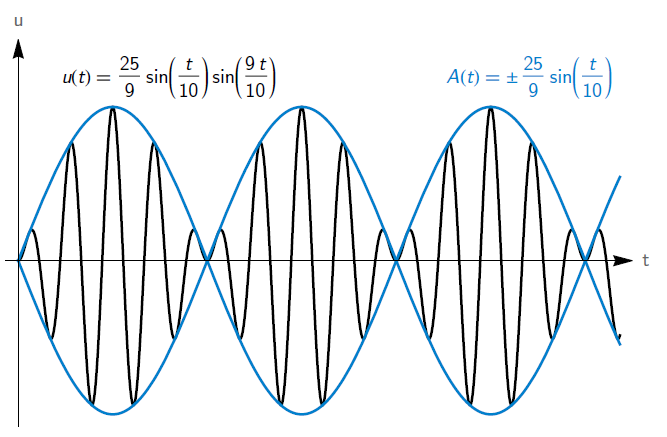
\includegraphics[width=10cm]{AN0.png}
\end{figure}

\end{block}
\end{frame}

\begin{frame}

$$y(t)=(A+x(t))\cos(\omega_ct+\theta_c),\hspace{3mm} A>|x(t)|_{\max}$$
\begin{figure}[h]
    \centering
    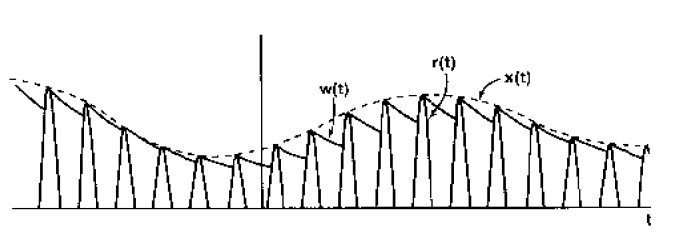
\includegraphics[width=10cm]{AM.png}
\end{figure}
\end{frame}




\end{document}
